\section {Implementation}

\subsection{Overview}
We implemented a small search engine that uses TweetRank to rank the tweets crawled from Twitter. The search engine has three main components: the crawler module, the \emph{ranker} module, and the Solr module. Figure \ref{fig:overview} represents the communication among the different components.

\begin{figure}
\centering
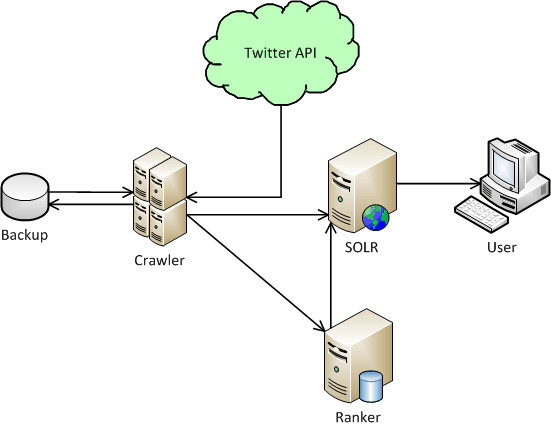
\includegraphics[width=0.4\textwidth]{../tweetmap.png} 
\caption{Overview of our search engine.}
\label{fig:overview}
\end{figure}

The crawler continuously fetches tweets from Twitter users using the Twitter API, saves the data to disk as a backup, parses it to extract the required information for our algorithms, and sends the parsed data to the ranker and the Solr module. The crawler sends the data to Solr using XML its XML POST request specification and it sends data to the ranker using a protocol designed by us. The crawler was designed to run in multiple threads or multiple machines.


\subsection{TweetRank}\label{sec:tweetrank_implementation}
Algorithm \ref{algo:alg1} is used to compute the TweetRank score and it is an adaptation of the classic Monte Carlo complete path stopping at dangling nodes method. The graph from Twitter $G$ is just the set of relationships described in section \ref{sec:tweetrank_definition}. Algorith \ref{algo:alg1} includes some predefined functions that are not described here, however we thought that their name is descriptive enough.

\begin{algorithm}
\caption{Compute TweetRank using MC complete path stopping at dangling nodes}
\label{algo:alg1}
{\fontsize{8}{8}\selectfont
\begin{algorithmic}
\REQUIRE Probabilities $\alpha, \beta, \gamma, \delta, \epsilon$ such that $\alpha+\beta+\gamma+\delta+\epsilon=1$, Twitter graph $G$ and $M \in \mathbb{N}$ such that $T\times M \in O(T^2)$.
\ENSURE $\pi$, TweetRank of tweets in $T(G)$.
\STATE $V_t \leftarrow 0, \forall t \in T$ \COMMENT{Visit counter for tweets}
\STATE $CP_0 \leftarrow \alpha$ \COMMENT{Cumulative probabilities for each action}
\FORALL{$t \in T(G)$}
\FOR {$m=1$ to $M$}
\STATE $ct \leftarrow t$
\STATE $stop \leftarrow False$
\WHILE {$\neg stop$}

\STATE $CP_1 \leftarrow CP_0 + \beta \cdot hasRetweetOrReply(ct)$
\STATE $CP_2 \leftarrow CP_1 + \gamma \cdot hasMentions(ct)$
\STATE $CP_3 \leftarrow CP_2 + \delta \cdot hasFriends(user(ct))$
\STATE $CP_4 \leftarrow CP_3 + \epsilon \cdot hasHashtags(ct)$

\STATE $r \leftarrow UniformRandomNumber(0, CP_4)$ \COMMENT{This ensures that all rows sums 1.0}

\IF { $r \leq CP_0$ }
\STATE $ct \leftarrow jumpToRandomTweet()$
\STATE $stop \leftarrow True$
\ELSIF { $r \leq CP_1$ }
\STATE $ct \leftarrow jumpToRetweetOrReply(ct)$
\ELSIF { $r \leq CP_2$ }
\STATE $ct \leftarrow jumpToMentionTweet(ct)$
\ELSIF { $r \leq CP_3$ }
\STATE $ct \leftarrow jumpToFriendTweet(ct)$
\ELSE
\STATE $ct \leftarrow jumpToHashtagTweet(ct)$
\ENDIF
\STATE $V_{ct} \leftarrow V_{ct} + 1$ 
\ENDWHILE
\ENDFOR
\ENDFOR
\STATE $\pi_t \leftarrow Normalize(V)$ \COMMENT{TweetRank as the normalized visit vector}
\end{algorithmic}}
\end{algorithm}

Observe that the running time of algorithm \ref{algo:alg1} is non-deterministic, since it depends on the structure of the graph itself and the $\alpha$ parameter. Assuming random access memory, and no dangling nodes in graph, the previous algorithm has an expected running time bounded by $O(|T| \times M \times \mathbb{E}[|w|])$, where $\mathbb{E}[|w|]$ is the expected length of the random walk. The expected length of the random walk is obtained from the following
equation:
\begin{equation}
\mathbb{E}[|w|] = \sum_{k=1}^{\infty} P(|w| = k) \cdot k = \sum_{k=1}^{\infty} (1 - \alpha)^{k-1} \cdot \alpha \cdot k = \frac{1}{\alpha}
\end{equation}

Given that $|T| \times M$ must be $O(|T|^ 2)$ to ensure a good approximation of TweetRank, the expected running time of algorithm \ref{algo:alg1} is:
\begin{equation}\label{eq:running_time}
O(|T| \times M \times \mathbb{E}[|w|]) = O(|T|^2 \times \frac{1}{\alpha}) = O(|T|^2)
\end{equation}

Note that equation \ref{eq:running_time} is an upper bound on the expected running time if the graph contains dangling nodes. On the other side, the assumption of random access memory might be a problem for a large index which does not fit in the main memory of a single machine. However, implementing TweetRank on a large-scale distributed system is not the approach of this work and we will made this assumption to keep the analysis simple.
%\subsection{HTTP server}

The Python crawler sends data using the POST request method in the HTTP protocol to the Java program which contains a HTTP server. For this to work, we have developed a simple protocol which these programs use to communicate. The protocol looks like this:

\begin{itemize}
	\item \textbf{Type} - The type of the data being sent.
	\begin{itemize}
		\item \textbf{RT} or \textbf{RP} - This tweet is a reply/retweet of the referenced tweet.
		\item \textbf{FW} - List of users that this user follows.
		\item \textbf{HT} - List of hashtags mentioned in this tweet.
		\item \textbf{MN} - List of users mentioned in this tweet.
		\item \textbf{TW} - List of tweets written by this user.
	\end{itemize}
	\item \textbf{ID} The ID of this user/tweet. (User for FW \& TW, tweet for all others.)
	\item \textbf{refID} Depends on the type.
	\begin{itemize}
		\item[] (RT/RP): Referenced tweet ID. Multiple IDs not allowed.
		\item[] (FW): User ID(s) that this user follows.
		\item[] (HT): Hashtag(s) mentioned in this tweet.
		\item[] (MN): User ID(s) of users that are mentioned in this tweet.
		\item[] (TW): Tweet ID(s) of tweets that are written by this user.
	\end{itemize}
\end{itemize}

\textit{Implementation note: all IDs are handled as numbers of type Long. refID for HT/Hashtag and the type parameter are handled as Strings.}

Upon successful parsing in the HTTP server, the data is sent to the ranker which adds it to the lists of already existing data. % Too extensive, I wouldn't talk about the crawler and the http server too much, just mention them in the overview.


\subsection{Solr - Incomplete!}
Solr 3.6 were used as the query interface for the TweetRank. It receives the Tweets from the Crawler by XML POST requests and indexes them. To improve the usability we also make use of the built-in tf-idf scoring that is offered by Solr/Lucene.

The TweetRank scores which are calculated at the ranker component which then prints the results as key value pairs in a plain text formatted file. This file is then used by Solr as an ''External file field'' which we combine with the other ranking attributes. The ranking attributes that we base our weighting on are the following:

\begin{itemize}
	\item \textbf{Hashtag} - If a hashtag $H$ is mentioned in the tweet $T$ and found in the query $Q$, we give additional score to $T$ for the query $Q$.
	\item \textbf{Username} - If the username of the author of tweet $T$ is found in query $Q$, we give additional score to $T$ for the query $Q$.
\end{itemize}

In addition to the the mentions above, we give an additional score to tweets that have been tweeted recently. The function we used for this additional date score is following: 

\begin{equation}
\frac{a}{m*x+b}
\end{equation}

where we have defined $x$ as the age of the tweet in milliseconds, $m = 3.16E^{-11}$, $a = 0.08$ and $b = 0.05$. 